\documentclass[10pt,a4paper]{article}
\usepackage[paper=a4paper, hmargin=1.5cm, bottom=1.5cm, top=3.5cm]{geometry}

\usepackage[utf8]{inputenc}
\usepackage[spanish]{babel}

\usepackage{mathtools}
\usepackage{amsmath}
\usepackage{amsfonts}
\usepackage{amssymb}

\usepackage{xcolor}
\usepackage{listingsutf8}
\usepackage{booktabs}
\usepackage{hyperref}

\usepackage{caption}
\usepackage{subcaption}

\usepackage{algpseudocode}
\usepackage{ifthen}
\usepackage{enumitem}

\usepackage{graphicx}
\usepackage{tikz}

\DeclarePairedDelimiter{\ceil}{\lceil}{\rceil}

%\let\NombreFuncion=\textsc
%\let\TipoVariable=\texttt

%\newcommand{\TipoFuncion}[3]{%
  %\NombreFuncion{#1}(#2) \ifx#3\empty\else $\to$ \res\,: \TipoVariable{#3}\fi%
%}

% set the default code style
\lstset{
    frame=tb, % draw a frame at the top and bottom of the code block
    tabsize=4, % tab space width
    showstringspaces=false, % don't mark spaces in strings
    numbers=left, % display line numbers on the left
    commentstyle=\color{green}, % comment color
    keywordstyle=\color{blue}, % keyword color
    stringstyle=\color{red} % string color
}

% mathy stuff
\newtheorem{theorem}{Theorem}[section]
\newtheorem{lemma}[theorem]{Lemma}
\newtheorem{proposition}[theorem]{Proposición}
\newtheorem{corollary}[theorem]{Corollary}

\newenvironment{proof}[1][Demostración]{\begin{trivlist}
\item[\hskip \labelsep {\bfseries #1}]}{\end{trivlist}}
\newenvironment{definition}[1][Definición]{\begin{trivlist}
\item[\hskip \labelsep {\bfseries #1}]}{\end{trivlist}}
\newenvironment{example}[1][Example]{\begin{trivlist}
\item[\hskip \labelsep {\bfseries #1}]}{\end{trivlist}}
\newenvironment{remark}[1][Remark]{\begin{trivlist}
\item[\hskip \labelsep {\bfseries #1}]}{\end{trivlist}}

\newcommand{\qed}{\nobreak \ifvmode \relax \else
      \ifdim\lastskip<1.5em \hskip-\lastskip
      \hskip1.5em plus0em minus0.5em \fi \nobreak
      \vrule height0.75em width0.5em depth0.25em\fi}

\title{Algoritmos y Estructuras de Datos III \\ TP3}

\newcommand{\order}[1]{$\mathcal{O}(#1)$}

\begin{document}

%% cover page

\maketitle

\bigskip

\begin{table}[h]
\centering
\begin{tabular}{|l l l|}
\hline
Integrante       & \multicolumn{1}{c}{LU}     & Correo electrónico        \\ \hline
Martin Baigorria & \multicolumn{1}{c}{575/14} & martinbaigorria@gmail.com \\ 
Federico Beuter & 827/13                      & federicobeuter@gmail.com \\
Juan Rinaudo & 864/13                      & jangamesdev@gmail.com \\ 
Mauro Cherubini & 835/13                      & cheru.mf@gmail.com \\ \hline
\end{tabular}
\end{table}

\vfill

\begin{center}
\textbf{Reservado para la cátedra}
\end{center}
\begin{table}[h]
\centering
\begin{tabular}{|l|l|l|}
\hline
Instancia       & Docente & Nota \\ \hline
Primera entrega &         &      \\ \hline
Segunda entrega &         &      \\ \hline
\end{tabular}
\end{table}

\newpage
\tableofcontents
\newpage

% end cover page

\section{Introducción}

\subsection{Definiciones}

Antes de enunciar el problema a resolver en este trabajo practico, es necesario definir algunos conceptos.

Sea $G = (V,E)$ un grafo simple:
\begin{definition}
Un conjunto $I \subseteq V$ es un \textit{conjunto independiente} de $G$ si no existe ningún eje de $E$ entre los vértices de $I$. Es decir, los ejes de $I$ no están conectados por las aristas de $G$.
\end{definition}

\begin{definition}
Un conjunto $D \subseteq V$ es un \textit{conjunto dominante} de G si todo vértice de $G$ esta en $D$ o bien tiene al menos un vecino que esta en $D$.
\end{definition}

\begin{definition}
Un conjunto \textit{conjunto independiente dominante} de $G$ es un conjunto independiente que a su vez es dominante del grafo G. Desde un conjunto independiente dominante se puede acceder a cualquier vértice del grafo $G$ con solo recorrer una arista desde uno de sus vértices.
\end{definition}

\begin{definition}
Un \textit{Conjunto Independiente Dominante Mínimo} (CIDM) es el conjunto independiente dominante de $G$ de mínima cardinalidad.
\end{definition}

Cada definición debería ser acompañada con un gráfico. Por ejemplo, podemos mostrar dos conjuntos independientes y dominantes del mismo grafo, donde uno ese el CIDM.

\subsection{Introducción}
En 1979, Garey y Johnson probaron que el problema de encontrar el CIDM de un grafo es un problema NP-Hard\footnote{M.R. Garey, D.S. Johnson, Computers and Intractability: A Guide to the Theory of NP-Completeness, Freeman and Company, San Francisco (1979).}.
El objetivo del trabajo es utilizar diferentes técnicas algorítmicas para resolver este problema. En un principio diseñaremos e implementaremos un algoritmo exacto para el mismo. Dada la complejidad del problema, luego propondremos diferentes algoritmos heurísticos para llegar a una solución que sea lo suficientemente buena a fines prácticos en un tiempo razonable.

Si recordamos el problema 3 del TP1, podemos ver claramente que el mismo es un caso particular del problema del conjunto independiente dominante optimo. Esto se debe a que el problema de los caballos imponía cierta estructura sobre el grafo en el que se efectuaba la búsqueda. El grafo en si no era completo, dado que cada casilla era representada por un nodo, y un caballo no podía acceder a los nodos adyacentes. El movimiento de los caballos se modelaba con aristas entre nodos. En cambio, el problema de encontrar el CIDM se aplica a cualquier tipo de grafo. Dado que el problema de los caballos era computacionalmente costoso, podemos inferir, como ya lo confirma la literatura, que este problema se resolverá en tiempo no polinomial.

\subsection{Maximalidad y dominancia}

Las siguientes proposiciones serán útiles a lo largo del trabajo:

\begin{proposition}
Sea M un conjunto independiente maximal de G. $\forall v \in G.V$, si $v \notin M \implies \exists u \in M$ tal que $u$ es adyacente a $v$. 
\end{proposition}

\begin{proof}
Por absurdo. Sea M un conjunto independiente maximal y $v \notin G.V$. $\not\exists u \in M$ tal que $u$ es adyacente a $v$. Por lo tanto, puedo agregar $v$ a $M$ y el conjunto va a seguir siendo independiente. Esto es absurdo, dado que el conjunto era maximal.
\end{proof}

\begin{proposition}
Dado $G(V,E)$, todo conjunto independiente maximal es un conjunto independiente dominante.
\end{proposition}

\begin{proof}
Sea $M$ un conjunto independiente maximal. Por la propiedad anterior, si $v \notin M \implies \exists u \in M$ tal que $u$ es adyacente a $v$. Por lo tanto, si $v \notin M$ entonces tiene algún vecino que esta en $M$. Esto significa que $M$ es dominante.
\end{proof}

\newpage

\subsection{Modelado}
Muchos problemas se pueden modelar con grafos y se pueden resolver mediante la búsqueda del conjunto independiente dominante mínimo.

\subsubsection{Planificador Urbano}

Supongamos que un planificador urbano esta diseñando una ciudad con muchos barrios. Con el objetivo de proveer un buen sistema de salud para los habitantes, el planificador determina que cada barrio debe tener que cruzar a lo sumo un barrio para acceder a un hospital publico. Aquí podemos modelar a cada barrio con un vértice, y representar la adyacencia entre barrios con una arista. Al obtener el CIDM, obtenemos la ubicación y la mínima cantidad de hospitales públicos necesarios para cumplir con los objetivos del planificador.
\newpage

\section{Algoritmo Exacto}

\subsection{Notacion}

Sea $\gamma(G)$ el numero de vertices en el conjunto CIDM.

\subsection{Cotas Superiores e Inferiores}

El problema de
\newpage
\subsection{Experimentacion}

Para la experimentacion de backtracking se tomo de 6 a 40 nodos, y para cada familia de grafos se tomaron diferentes parametros para la misma cantidad de nodos. Los resultados fueron los siguientes:\\

\begin{figure}[ht]
\centering
	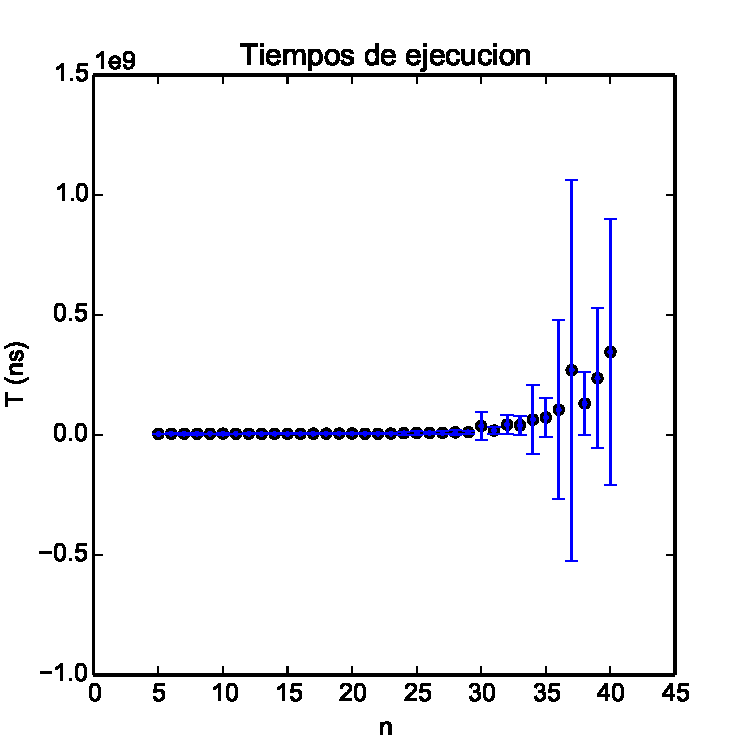
\includegraphics[scale=0.45]{images/graph_ej1/output_backtracking_1_n2}
	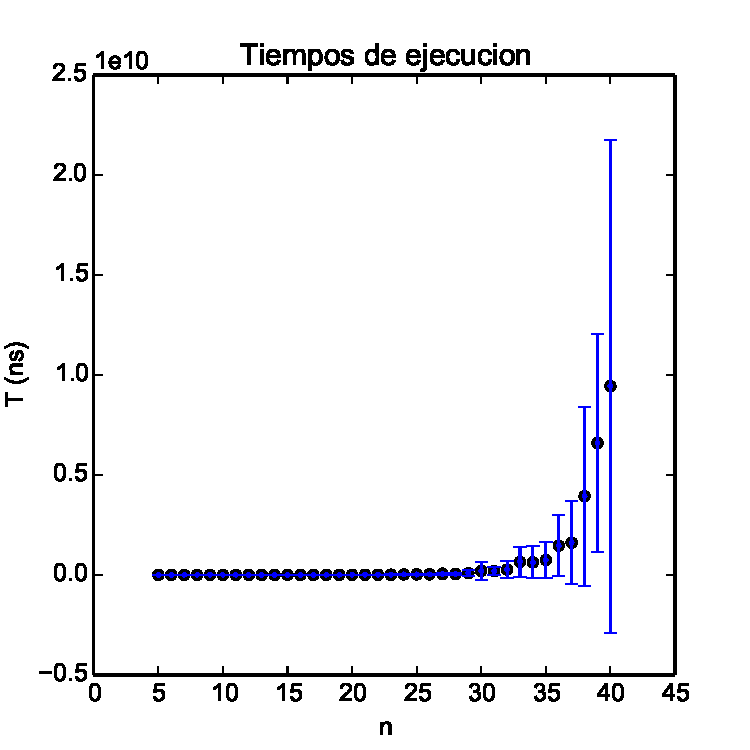
\includegraphics[scale=0.45]{images/graph_ej1/output_backtracking_1_n}
	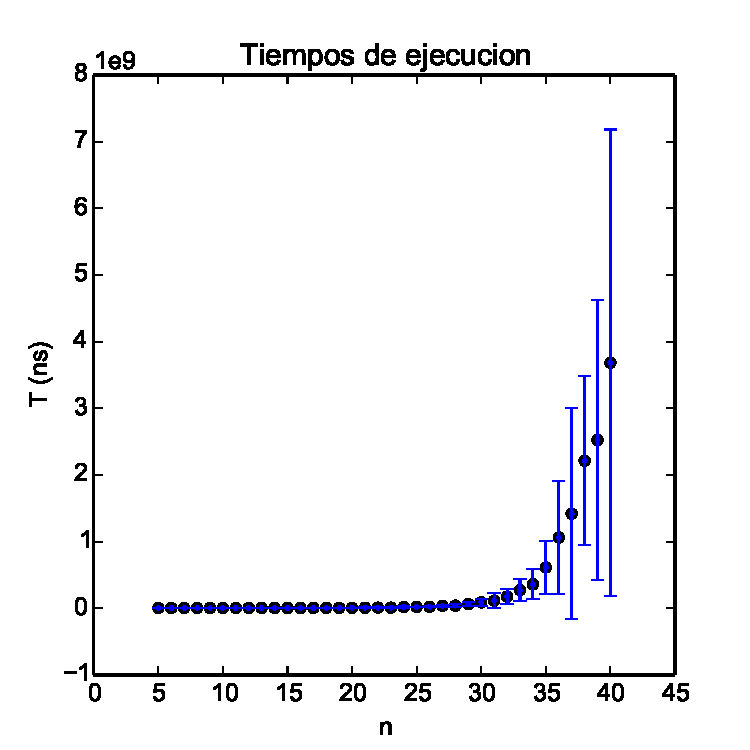
\includegraphics[scale=0.45]{images/graph_ej1/output_backtracking_1_2n}
\end{figure}
\newpage
\subsection{Codigo}
\lstinputlisting[language=C++, breaklines=true]{../src/backtracking/backtracking.cpp}
\newpage

\section{Heurística Constructiva Golosa}

\subsection{Algoritmos}

Dado que el problema de buscar el CIDM es NP-Hard, para este algoritmo resolveremos el problema por medio de una heurística golosa. La idea básicamente fue ir seleccionando nodos bajo algún criterio, agregándolos al conjunto solución y descartando todos los otros nodos que romperían la independencia de la potencial solución condicional al nodo agregado. Al quedarnos sin nodos para elegir, finalmente tendríamos un conjunto independiente y dominante válido. Dado que la heurística no siempre es optima, muchas veces sucederá que este conjunto que encontraremos no sera el mínimo. Este procedimiento se puede ver en el siguiente pseudocódigo: Para elegir que nodo seleccionar dado los nodos disponibles, utilizaremos la selección por \texttt{grado} y por \texttt{scoring}, que explicaremos a continuación.


\subsubsection{Por grado}

\subsubsection*{Criterio}

Al principio decidimos implementar este criterio de selección de nodos utilizando un heap, ordenando los nodos por su grado. Esto se puede hacer facilmente con el algoritmo de Floyd en Luego, desencolamos del heap y vamos actualizando los flags de cada nodo a medida que son alcanzables. El algoritmo tiene \order{n \times log(n) + m}.

\subsubsection*{Pseudocodigo}

\begin{algorithmic}
\Procedure{greedyHeapConstructive}{G}

\State{nodeHeap $\gets$ buildHeap(G.V)}

\While{!nodeHeap.isEmpty()}
	\State{node $\gets$ nodeHeap.pop()}
	\If{node.reachable == true}
		\State{continue}
	\EndIf
	\State{node.added = true}
	
	\ForAll{$adj \in node.adj$}
		\State{adj.reachable $\gets$ true}
	\EndFor
\EndWhile
\EndProcedure
\end{algorithmic}

\subsubsection{Scoring}

\subsubsection*{Criterio}

Aunque este método con el heap es rápido, en realidad podemos mejorar la forma en la que seleccionamos los vértices. Este método consiste en tomar el número de nodos adyacentes efectivos (score) a los que cada nodo puede acceder. Definimos a un nodo adyacente efectivo como un nodo que es adyacente y a su vez no puede ser accedido por otros nodos que ya pertenecen a la solución parcial en construcción. De esta forma, este criterio también nos garantiza la independencia del conjunto, dado que si tomamos dos nodos de la solución, por construcción no pueden ser adyacentes.

Cada nodo va a tener como atributos su score, un flag que indica si ha sido agregado y otro que indica si es alcanzable por el cubrimiento parcial actual.

El algoritmo va a iterar un arreglo de nodos $n^2$ veces. Cada vez que busquemos un nodo para agregar al conjunto, los iteraremos todos para buscar el de máximo score. Al identificarlo, actualizaremos los scores de los nodos adyacentes a los adyacentes del mismo. A priori parece que la complejidad de este nuevo algoritmo se podría mejorar de forma significativa utilizando algún otro tipo de estructura de datos.

\subsubsection*{Pseudocodigo}

\begin{algorithmic}
\Procedure{greedyConstructive}{G}

\For{i = 0 to i $<$ G.size() }

	\State{greatest $\gets$ 0}
	\State{score $\gets$ 0}
	\State{flag $\gets$ false}

	\For{j = 0 to j $<$ G.size() }
		\If{graph[j] == true}
			\State{continue}
		\EndIf
		\If{graph[j].score $\geq$ score}
			\State{greatest $\gets$ j}
			\State{score $\gets$ graph[j].score}
			\State{flag $\gets$ true}
		\EndIf
	\EndFor

	\If{!flag} \State{break} \EndIf
	
	\State{graph[greatest].added $\gets$ true}
	\State{graph[greatest].reachable $\gets$ true}
	
	\ForAll{$adjNode \in graph[greatest].adj$}
		\State{adjNode.reachable $\gets$ true}
		\ForAll{$adjToAdj \in adjNode.adj$}
			\State{adjToAdj.score--}
		\EndFor
	\EndFor
	
\EndFor
\EndProcedure
\end{algorithmic}

\subsection{Complejidad}

El primer algoritmo resuelve el problema en \order{n \times log(n) + m} simplemente ignorando la actualización de los scores, desencolando de un heap $n$ veces. Sin embargo, este criterio es a simple vista inferior que el de actualización de scores. Aquí hay un tradeoff entre hacer la mejor elección y la complejidad temporal del algoritmo.

El algoritmo basado en el score recorre arreglo $n$ veces. A su vez, buscar los adyacentes de los adyacentes se hace $m$ veces en total. Luego actualizamos en total el score de $m$ nodos. Por lo tanto, el algoritmo tiene orden \order{n^2 + 2 \times m}, es decir \order{n^2}.

Notar que la forma en que buscamos el máximo es sumamente ineficiente. Esto se debe a que si utilizamos sort, luego es bastante difícil encontrar el nodo al que le debemos actualizar su respectivo score. A su vez, dado que en cada iteración actualizamos el score, mantener el orden es sumamente costoso. Es muy posible que exista una estructura de datos mucho más eficiente para resolver este problema (una especie de heap dinámico), aunque para este trabajo practico nos conformaremos con el algoritmo en \order{n^2}.

\subsection{Efectividad de la heurística}

Nuestra heurística no siempre devuelve la solución optima. Considerar los siguientes ejemplos:

\begin{figure}[ht]
\centering
\begin{subfigure}[b]{0.4\textwidth}
	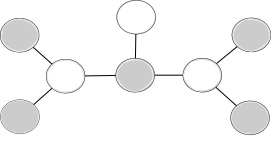
\includegraphics[scale=0.6]{images/greedy_fail.png}
	\caption{Greedy (5 nodos)}
\end{subfigure}
\begin{subfigure}[b]{0.4\textwidth}
	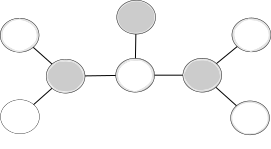
\includegraphics[scale=0.6]{images/greedy_best.png}
	\caption{Óptimo (3 nodos)}
\end{subfigure}

\begin{subfigure}[b]{0.4\textwidth}
	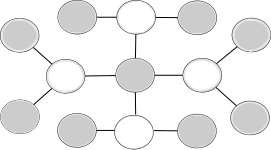
\includegraphics[scale=0.6]{images/greedy_fail2.png}
	\caption{Greedy (9 nodos)}
\end{subfigure}
\begin{subfigure}[b]{0.4\textwidth}
	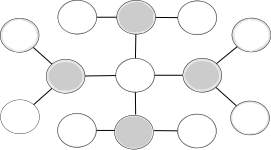
\includegraphics[scale=0.6]{images/greedy_best2.png}
	\caption{Óptimo (4 nodos)}
\end{subfigure}
\caption{Ejemplos de nuestra heurística comparado con el óptimo.}
\end{figure}

El peor caso es claramente el de la figura (c) y (d). Tenemos un nodo $v$ (el nodo central) de grado $d(v) = 4$, con sus nodos adyacentes de grado $d(u) = 3$. Si tenemos $c$ componentes conexas de ese tipo, utilizaremos $c \times (2 \times 4 + 1)$ nodos, cuando en realidad el optimo tiene $c \times 4$ nodos.




\newpage

\section{Heurística de Búsqueda Local}

\subsection{Algoritmo}

Antes de explicar nuestro algoritmo, comenzemos definiendo que es una heurística de búsqueda local. Para cada solución factible $s \in S$, se define $N(s)$ como el conjunto de soluciones vecinas de $s$. Un procedimiento de búsqueda local toma una solución inicial $s$ e iterativamente la mejora reemplazándola por otra solución mejor del conjunto $N(s)$, hasta llegar a un optimo local. El algoritmo se puede ver con el siguiente pseudocodigo:

\begin{algorithmic}
\Procedure{localSearch}{G}
\State{s $\gets$ getInitialSolution(G)}
\State{localSolution $\gets$ true}
\While{localSolution}
	\State{$localSolution \gets false$}
	\ForAll{$\hat{s} \in N(s)$}
		\If{$|\hat{s}| < |s|$}
			\State{$s \gets \hat{s}$}
			\State{$localSolution \gets true$}
			\State{break}
		\EndIf
	\EndFor
\EndWhile
\EndProcedure
\end{algorithmic}

\hspace{1px}

En primer lugar hay que pensar que algoritmo utilizar en la función $getInitialSolution(G)$. Para esto, utilizamos cualquiera de las heurísticas constructivas golosas del paso anterior.

Luego, debemos identificar como construiremos las diferentes $s \in N(s)$, es decir, como construiremos la función que nos devuelve los vecinos de una solución parcial $N(S)$.

\subsection{Vecindades}

Para este algoritmo, utilizaremos los siguientes dos criterios para definir la vecindad de una solución $s$:

\begin{enumerate}
\item \underline{Primera vecindad:}
Para la primera vecindad simplemente tomamos un vértice que actualmente no pertenece a la solución local. Luego, quitamos todos sus vértices adyacentes y verificamos si tenemos una solución con menor cardinal.
\item \underline{Segunda vecindad:}
Para este criterio, lo que hacemos es buscar dos nodos que no pertenecen a la solución local. Los agregamos, quitamos sus nodos adyacentes, y verificamos si el nuevo conjunto es un cubrimiento de menor cardinal.
\end{enumerate}

\subsection{Complejidad}

\subsubsection{Primera vecindad}

En una iteración, el primer algoritmo de vecindad agrega un nodo y luego quita sus adyacentes. Luego verifica que los adyacentes de estos vértices que hemos quitado son alcanzables. Por lo tanto, en el peor caso una iteración tiene orden \order{n \times \Delta(G)^3}. Esto se debe a que se debe verificar que todos los nodos adyacentes a los que saque son adyacentes a algún otro nodo del conjunto en \order{\Delta(G)} para cada nodo adyacente ($\Delta(G)$) a los adyacentes que pude quitar ($\Delta(G)$). Si el nuevo conjunto de nodos no es un CIDM, simplemente restauramos el grafo en \order{\Delta(G)}.

\subsubsection{Segunda vecindad}

En el segundo caso, probamos agregando todos los pares de nodos a la solución actual, quitando sus nodos adyacentes y verificando si luego es una solución. Para ello, simplemente repetimos el procedimiento de la primera vecindad.

Este procedimiento lo repetimos para todo par de $v \not\in S$. Podemos acotar esto de forma grotesca por $\binom{n}{2}$. Por lo tanto la complejidad total de una iteración es de \order{\binom{n}{2} \times \Delta(G)^3}.

\newpage

\section{Metaheurística GRASP}

\subsection{Algoritmo}

\subsection{Complejidad}

\end{document}